\documentclass{article}

\usepackage{graphicx}
\usepackage{tikz}
\usepackage{tikzsymbols}
\usetikzlibrary{calc,patterns,shapes.geometric}
\pagestyle{empty}
\usepackage[margin=0pt]{geometry}
\geometry{papersize={14in,12in}}

\def\centerarc[#1](#2)(#3:#4:#5){\draw[#1] ($(#2)+({#5*cos(#3)},{#5*sin(#3)})$) arc (#3:#4:#5);}

\begin{document}
	\begin{figure}
		\centering
		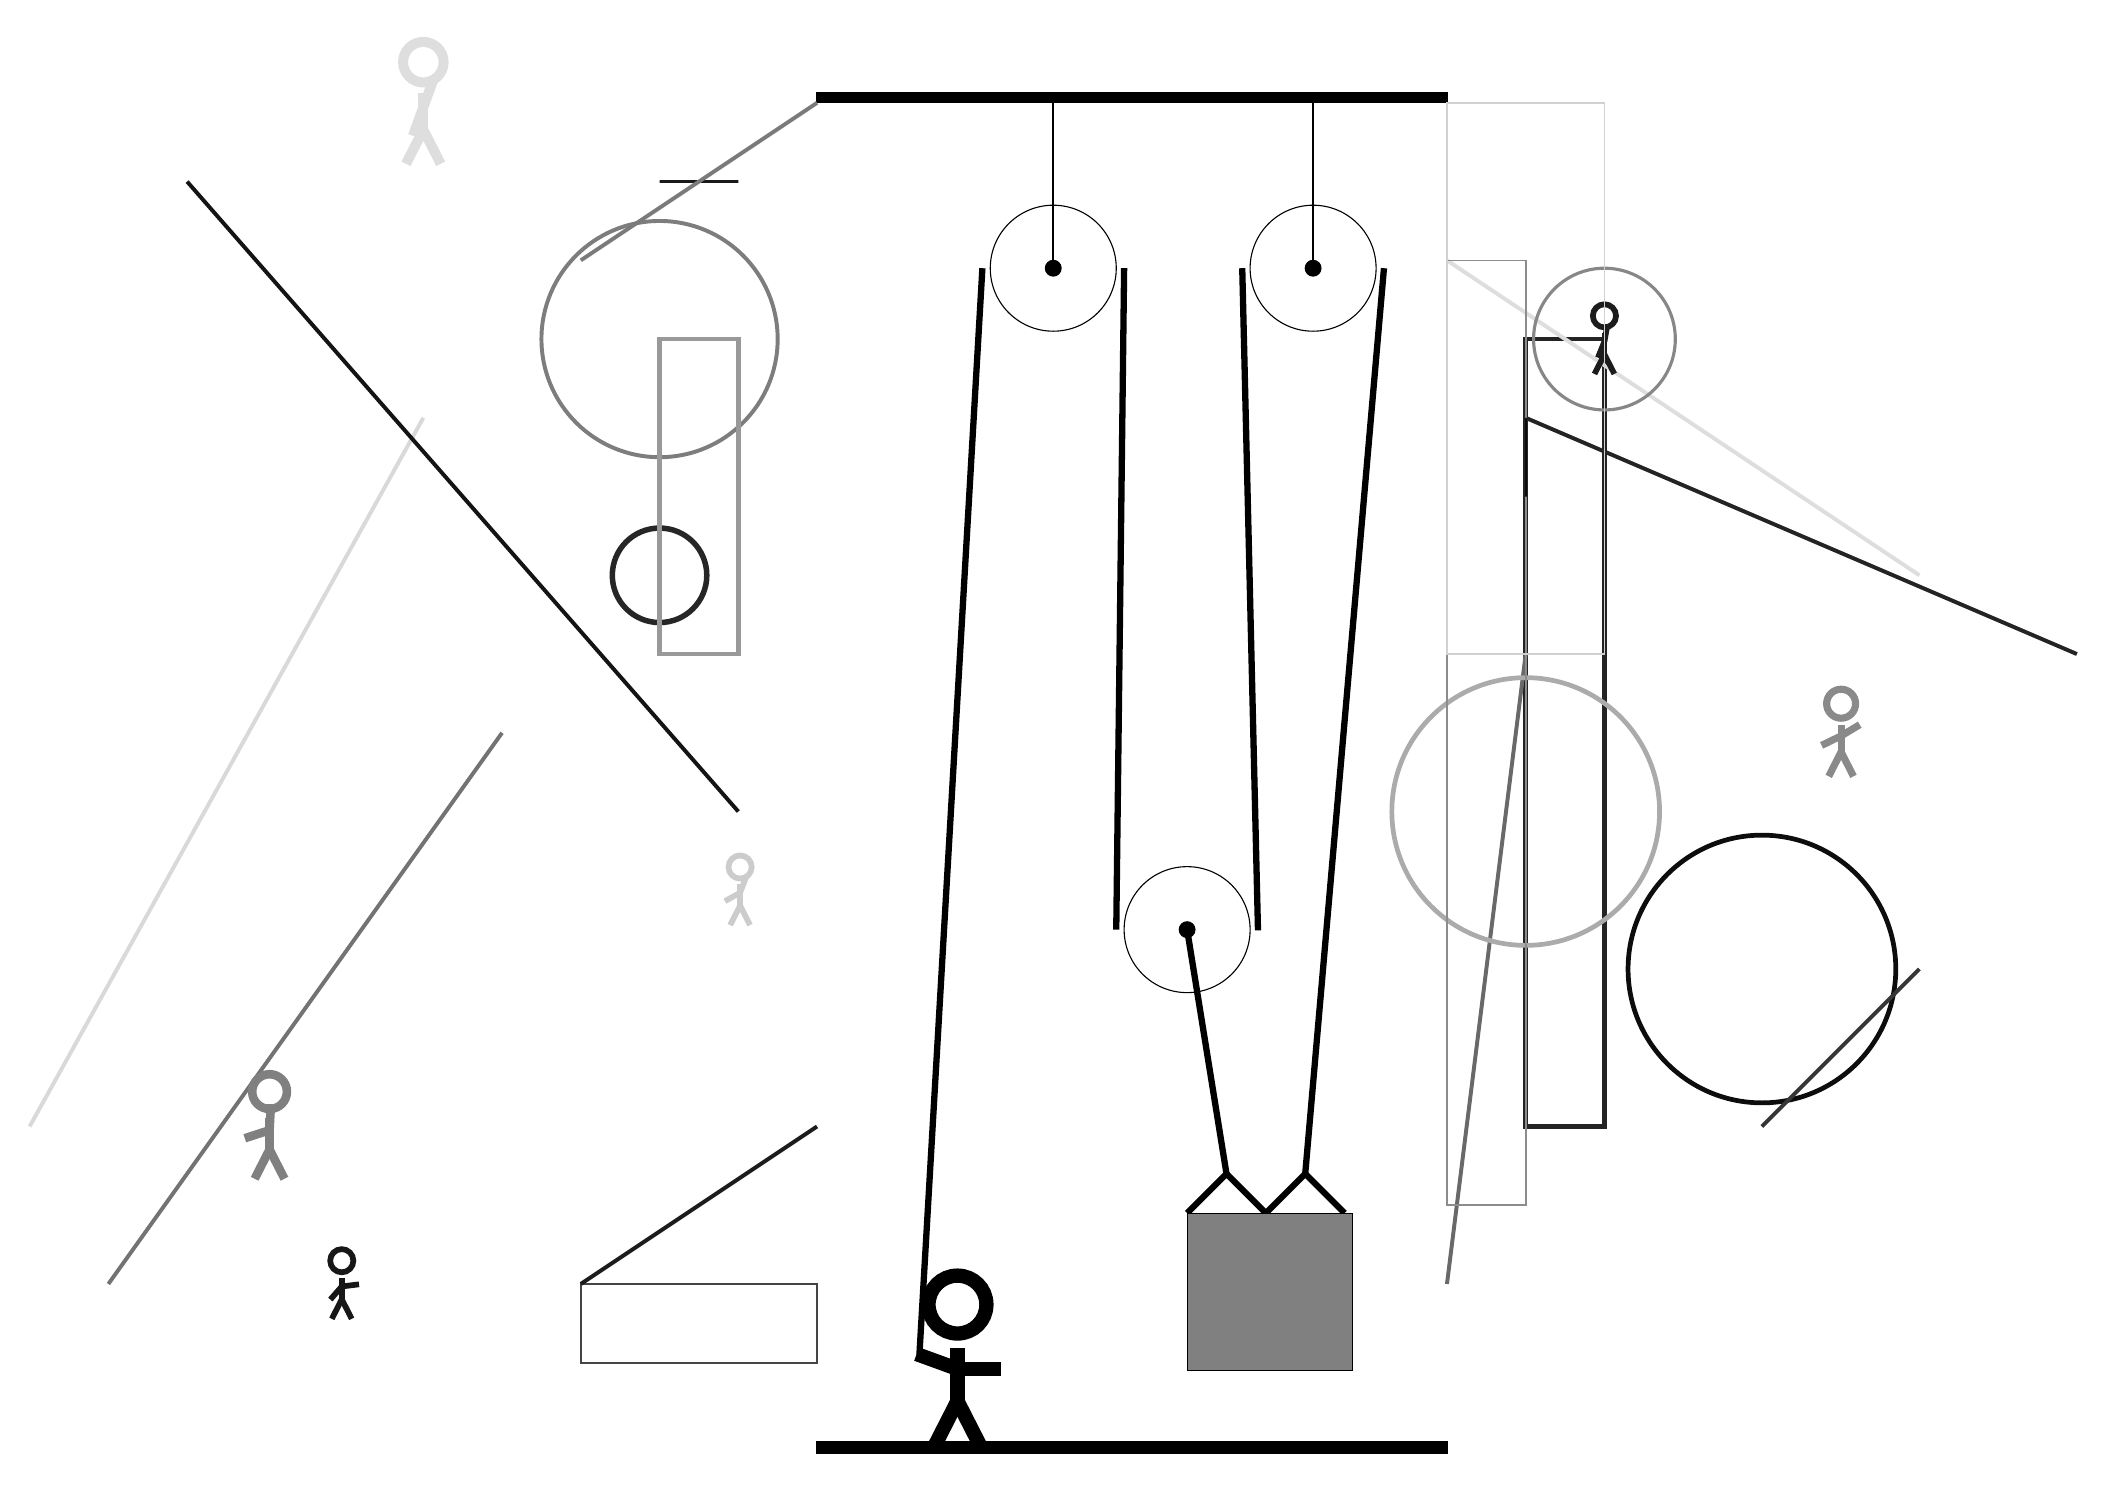
\begin{tikzpicture}
			%%%%% START %%%%%
			
			\draw[fill=black] (-2, 14) rectangle (6, 14.125);
			
			\draw (1, 11.9) circle (0.8);
			\draw[fill=black] (1, 11.9) circle (0.1);
			\draw[thick] (1, 11.9) -- (1, 14);
			
			\draw (4.3, 11.9) circle (0.8);
			\draw[fill=black] (4.3, 11.9) circle (0.1);
			\draw[thick] (4.3, 11.9) -- (4.3, 14);
			
			\draw (2.7, 3.5) circle (0.8);
			\draw[fill=black] (2.7, 3.5) circle (0.1);
			
			\draw[line width=0.8mm]  (2.7, -0.1) -- (3.2, 0.4) -- (3.7, -0.1) -- (4.2, 0.4) -- (4.7, -0.1);
			\draw[fill=black!50] (2.7, -0.1) rectangle (4.8, -2.1);
			
			\draw [line width=0.7mm, color=black!85](-4, 8) circle (0.6);
			
			\draw[line width=0.6mm, color=black!86] (7, 11) rectangle (8, 1);
			\draw[line width=0.5mm, color=black!86](7, 10) -- (14, 7);
			\draw[line width=0.2mm, color=black!73] (-2, -2) rectangle (-5, -1);
			\draw [line width=0.5mm, color=black!51](-4, 11) circle (1.5);
			\draw [line width=0.6mm, color=black!95](10, 3) circle (1.7);
			\draw[line width=0.5mm, color=black!59](7, 7) -- (6, -1);
			
			\node[line width=0.2mm, color=black!20] at (-3, 4) {\Strichmaxerl[4][29][69]};
			\node[line width=0.2mm, color=black!46] at (11, 6) {\Strichmaxerl[5][26][31]};
			
			\draw[line width=0.5mm, color=black!55](-6, 6) -- (-11, -1);
			
			\draw[line width=0.6mm, color=black!40] (-4, 7) rectangle (-3, 11);
			
			\draw [line width=0.6mm, color=black!33](7, 5) circle (1.7);
			\node[line width=0.2mm, color=black!50] at (-9, 1) {\Strichmaxerl[6][18][87]};
			
			\draw[line width=0.5mm, color=black!13](6, 12) -- (12, 8);
			\draw[line width=0.2mm, color=black!45] (6, 12) rectangle (7, 0);
			\draw[line width=0.3mm, color=black!90] (-4, 13) rectangle (-3, 13);
			\draw[line width=0.5mm, color=black!15](-7, 10) -- (-12, 1);
			
			\draw [line width=0.4mm, color=black!47](8, 11) circle (0.9);
			\draw[line width=0.5mm, color=black!89](-5, -1) -- (-2, 1);
			
			\draw[line width=0.5mm, color=black!52](-2, 14) -- (-5, 12);
			\node[line width=0.2mm, color=black!89] at (8, 11) {\Strichmaxerl[4][68][80]};
			\draw[line width=0.2mm, color=black!18] (8, 7) rectangle (6, 14);
			
			\draw[line width=0.5mm, color=black!92](-3, 5) -- (-10, 13);
			\draw[line width=0.5mm, color=black!79](10, 1) -- (12, 3);
			\node[line width=0.7mm, color=black!13] at (-7, 14) {\Strichmaxerl[7][70][70]};
			
			\node[line width=0.2mm, color=black!91] at (-8, -1) {\Strichmaxerl[4][49][7]};
			
			\draw[line width=0.3mm, color=black!95] (7, 9) rectangle (7, 10);
			
			\draw[line width=0.8mm](-0.7, -1.9) -- (0.1, 11.9);
			\centerarc[line width=0.8mm](1, 11.9)(0:180:0.9);
			\draw[line width=0.8mm](1.9, 11.9) -- (1.8, 3.5);
			\centerarc[line width=0.8mm](2.7, 3.5)(180:370:0.9);
			\draw[line width=0.8mm] (3.6, 3.49) -- (3.4, 11.9);
			\centerarc[line width=0.8mm](4.3, 11.9)(0:180:0.9);
			\draw[line width=0.8mm](4.2, 0.4) -- (5.2, 11.9);
			\draw[line width=0.8mm] (3.2, 0.4) -- (2.7, 3.5);
			
			\node at (-0.2, -2) {\Strichmaxerl[10][-20][0]};
			
			\draw[fill=black] (-2, -3) rectangle (6, -3.15);
			
			%%%%% END %%%%%
		\end{tikzpicture}
	\end{figure}	
\end{document}